%============================================================
% CHAPITRE V — Résultats, généricité et perspectives
%============================================================
\chapter{Résultats, généricité et perspectives}

\section*{Sommaire}
\begin{quote}
\small
\textbf{V.1} \hspace{1em} Introduction \dotfill \pageref{sec:intro_ch5}\\
\textbf{V.2} \hspace{1em} Stratégie de tests \dotfill \pageref{sec:test_strat}\\
\hspace{2.5em} V.2.1 \hspace{0.5em} Objectifs des tests \dotfill \pageref{subsec:test_obj}\\
\hspace{2.5em} V.2.2 \hspace{0.5em} Tests unitaires \dotfill \pageref{subsec:unit}\\
\hspace{2.5em} V.2.3 \hspace{0.5em} Tests d'intégration \dotfill \pageref{subsec:integ}\\
\hspace{2.5em} V.2.4 \hspace{0.5em} Tests de robustesse \dotfill \pageref{subsec:robust}\\
\hspace{2.5em} V.2.5 \hspace{0.5em} Critères d'acceptation \dotfill \pageref{subsec:accept}\\
\textbf{V.3} \hspace{1em} Tests des services core \dotfill \pageref{sec:core_tests}\\
\hspace{2.5em} V.3.1 \hspace{0.5em} Tests du module Config \dotfill \pageref{subsec:t_config}\\
\hspace{2.5em} V.3.2 \hspace{0.5em} Tests du module Storage \dotfill \pageref{subsec:t_storage}\\
\hspace{2.5em} V.3.3 \hspace{0.5em} Tests du module Logger \dotfill \pageref{subsec:t_logger}\\
\hspace{2.5em} V.3.4 \hspace{0.5em} Tests du module Diagnostic \dotfill \pageref{subsec:t_diag}\\
\hspace{2.5em} V.3.5 \hspace{0.5em} Tests de configuration corrompue \dotfill \pageref{subsec:t_corrupt}\\
\hspace{2.5em} V.3.6 \hspace{0.5em} Tests de log plein \dotfill \pageref{subsec:t_logfull}\\
\textbf{V.4} \hspace{1em} Tests système et scénarios critiques \dotfill \pageref{sec:sys_tests}\\
\hspace{2.5em} V.4.1 \hspace{0.5em} Test de reboot \dotfill \pageref{subsec:t_reboot}\\
\hspace{2.5em} V.4.2 \hspace{0.5em} Test incident vers safe mode \dotfill \pageref{subsec:t_safe}\\
\hspace{2.5em} V.4.3 \hspace{0.5em} Test de reprise après reboot \dotfill \pageref{subsec:t_resume}\\
\hspace{2.5em} V.4.4 \hspace{0.5em} Test config/diag via canal réel \dotfill \pageref{subsec:t_canal}\\
\hspace{2.5em} V.4.5 \hspace{0.5em} Test du sélecteur de protocole sur mocks \dotfill \pageref{subsec:t_proto}\\
\textbf{V.5} \hspace{1em} Profiling mémoire et durcissement \dotfill \pageref{sec:profiling}\\
\hspace{2.5em} V.5.1 \hspace{0.5em} Mesure de la mémoire RAM \dotfill \pageref{subsec:ram}\\
\hspace{2.5em} V.5.2 \hspace{0.5em} Mesure des stacks FreeRTOS \dotfill \pageref{subsec:stacks}\\
\hspace{2.5em} V.5.3 \hspace{0.5em} Règles d'allocation mémoire \dotfill \pageref{subsec:alloc}\\
\hspace{2.5em} V.5.4 \hspace{0.5em} Garde-fous mémoire \dotfill \pageref{subsec:guards}\\
\hspace{2.5em} V.5.5 \hspace{0.5em} Nettoyage des APIs \dotfill \pageref{subsec:apiclean}\\
\hspace{2.5em} V.5.6 \hspace{0.5em} Refactor léger \dotfill \pageref{subsec:refactor}\\
\textbf{V.6} \hspace{1em} Release candidate du noyau firmware \dotfill \pageref{sec:release}\\
\hspace{2.5em} V.6.1 \hspace{0.5em} Stabilisation du code \dotfill \pageref{subsec:stab}\\
\hspace{2.5em} V.6.2 \hspace{0.5em} Vérification de la compilation CI \dotfill \pageref{subsec:ci_verif}\\
\hspace{2.5em} V.6.3 \hspace{0.5em} Vérification de la documentation API \dotfill \pageref{subsec:doc_verif}\\
\hspace{2.5em} V.6.4 \hspace{0.5em} Préparation d'une version transférable \dotfill \pageref{subsec:transfer_ver}\\
\textbf{V.7} \hspace{1em} Documentation finale et transfert \dotfill \pageref{sec:docs}\\
\hspace{2.5em} V.7.1 \hspace{0.5em} Documentation d'architecture \dotfill \pageref{subsec:doc_archi}\\
\hspace{2.5em} V.7.2 \hspace{0.5em} Documentation des modules \dotfill \pageref{subsec:doc_mods}\\
\hspace{2.5em} V.7.3 \hspace{0.5em} Guide d'ajout d'un driver \dotfill \pageref{subsec:doc_driver}\\
\hspace{2.5em} V.7.4 \hspace{0.5em} Guide de configuration \dotfill \pageref{subsec:doc_cfg}\\
\hspace{2.5em} V.7.5 \hspace{0.5em} Guide de tests \dotfill \pageref{subsec:doc_tests}\\
\hspace{2.5em} V.7.6 \hspace{0.5em} Dossier de transfert final \dotfill \pageref{subsec:doc_transfer}\\
\textbf{V.8} \hspace{1em} Discussion des résultats \dotfill \pageref{sec:discussion}\\
\textbf{V.9} \hspace{1em} Conclusion \dotfill \pageref{sec:conclu_ch5}\\
\end{quote}

\newpage

%============================================================
\section{Introduction}
\label{sec:intro_ch5}
%============================================================

Ce chapitre constitue le bilan final du projet de développement du
firmware générique \textit{GlobalFleet}. Il s'articule en quatre axes
complémentaires dont l'objectif commun est de démontrer que le firmware
conçu et implémenté répond effectivement aux six catégories d'exigences
identifiées au chapitre~III et satisfait les critères industriels
définis en début de projet avec l'équipe de Smart Automation Technologies.

Le premier axe est la validation par les tests : une stratégie de
tests structurée en trois niveaux — unitaire, intégration et
robustesse — permet de vérifier que chaque composant se comporte
conformément à son interface contractuelle, et que le système dans
son ensemble gère correctement les scénarios d'erreur critiques
identifiés en déploiement industriel : corruption de configuration,
saturation du stockage, perte de connectivité prolongée et boucles
de redémarrages. Les tests s'appuient sur le répertoire
\texttt{test\_host/} pour les validations hors-cible et sur le
répertoire \texttt{test/} pour les validations sur cible réelle
ESP32-P4.

Le deuxième axe est l'analyse quantitative des résultats : les mesures
de consommation mémoire heap, de profil des stacks FreeRTOS par tâche,
et les résultats chiffrés des scénarios de test permettent d'évaluer
l'adéquation du firmware aux contraintes industrielles définies dans
les critères d'acceptation. Les résultats numériques sur cible seront
complétés dès réception du matériel ESP32-P4 ; les emplacements
correspondants sont signalés explicitement dans les sections suivantes.

Le troisième axe concerne la stabilisation et le transfert : la
préparation de la \textit{release candidate} du noyau firmware, la
vérification de la documentation API générée par Doxygen et la
constitution du dossier de transfert garantissent la maintenabilité
et la reprise du projet par l'équipe R\&D de SAT au-delà de la période
de stage. Le quatrième axe est prospectif : une discussion honnête
des apports et des limites de l'architecture, suivie des perspectives
d'évolution concrètes, ouvre des pistes documentées pour les prochaines
versions du produit.

%============================================================
\section{Stratégie de tests}
\label{sec:test_strat}
%============================================================

%------------------------------------------------------------
\subsection{Objectifs des tests}
\label{subsec:test_obj}
%------------------------------------------------------------

La stratégie de tests du firmware \textit{GlobalFleet} vise trois
objectifs distincts et complémentaires, correspondant aux trois niveaux
de confiance nécessaires avant une release candidate industrielle.
Le premier objectif est la vérification de la conformité fonctionnelle
de chaque module par rapport à son interface contractuelle définie au
chapitre~III : chaque fonction publique exportée doit se comporter
exactement comme documenté dans les fichiers \texttt{.h}, y compris
dans les cas limites et les cas d'erreur. Le deuxième objectif est
la validation du comportement du système dans les scénarios dégradés
les plus critiques en déploiement industriel : corruption de
configuration NVS, saturation du stockage Flash, dépassement du
timeout watchdog d'une tâche, et succession rapide de redémarrages
déclenchant le mécanisme anti-boucle. Le troisième objectif est la
mesure des indicateurs de performance quantitatifs — consommation
mémoire heap, marges de stack FreeRTOS, latence du bus d'événements,
temps de transitions FSM — et leur vérification de conformité aux
critères d'acceptation définis dans le tableau~\ref{tab:acceptance}.

%------------------------------------------------------------
\subsection{Tests unitaires}
\label{subsec:unit}
%------------------------------------------------------------

Les tests unitaires sont implémentés avec le framework Unity~2.5.2,
exécutés hors-cible sur machine de développement (\textit{host-side
testing}) depuis le répertoire \texttt{test\_host/}, et sur cible
depuis le répertoire \texttt{test/} (\texttt{test\_subscription\_manager.c}).
Cette dualité d'exécution est essentielle : les tests hors-cible
s'exécutent en quelques secondes dans le pipeline CI, tandis que les
tests sur cible valident les comportements dépendant du matériel
réel (timing FreeRTOS, accès NVS, interruptions GPIO). Chaque
composant possède son propre ensemble de tests couvrant les cas
nominaux, les cas limites (valeurs en frontière de plage) et les cas
d'erreur (valeurs invalides, ressources épuisées). Les dépendances
vers les drivers HAL sont substituées par des stubs injectables via
des pointeurs de fonctions, permettant de simuler n'importe quelle
condition d'erreur driver de manière déterministe et reproductible.

\begin{figure}[H]
\centering
\resizebox{0.85\textwidth}{!}{%
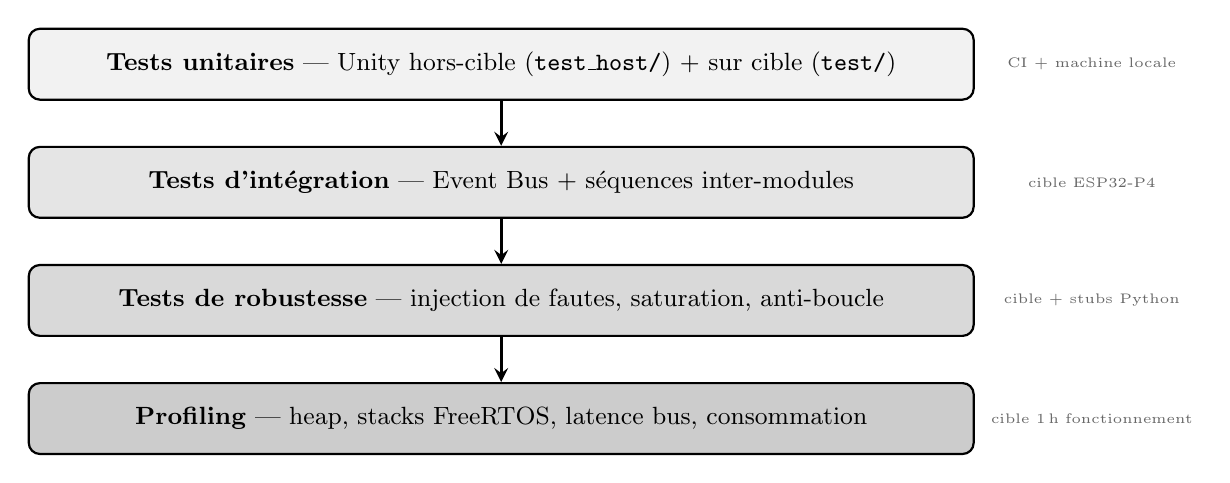
\begin{tikzpicture}[font=\small,
  level/.style={
    draw, rounded corners=4pt,
    minimum width=12cm,
    minimum height=0.9cm,
    align=center,
    fill=#1,
    text=black,
    thick
  },
  arr/.style={->, very thick, >=stealth, black}
]
  \node[level=gray!10]  (unit)  at (0, 0)
        {\textbf{Tests unitaires} — Unity hors-cible (\texttt{test\_host/}) + sur cible (\texttt{test/})};
  \node[level=gray!20]  (integ) at (0,-1.5)
        {\textbf{Tests d'intégration} — Event Bus + séquences inter-modules};
  \node[level=gray!30]  (rob)   at (0,-3.0)
        {\textbf{Tests de robustesse} — injection de fautes, saturation, anti-boucle};
  \node[level=gray!40]  (perf)  at (0,-4.5)
        {\textbf{Profiling} — heap, stacks FreeRTOS, latence bus, consommation};
  \draw[arr] (unit) -- (integ);
  \draw[arr] (integ) -- (rob);
  \draw[arr] (rob) -- (perf);
  % Annotations droite
  \node[font=\tiny, black!60, align=left] at (7.5,  0)   {CI + machine locale};
  \node[font=\tiny, black!60, align=left] at (7.5, -1.5) {cible ESP32-P4};
  \node[font=\tiny, black!60, align=left] at (7.5, -3.0) {cible + stubs Python};
  \node[font=\tiny, black!60, align=left] at (7.5, -4.5) {cible 1\,h fonctionnement};
\end{tikzpicture}%
}
\caption{Pyramide de tests du firmware \textit{GlobalFleet} — quatre niveaux progressifs}
\label{fig:test_pyramid}
\end{figure}

%------------------------------------------------------------
\subsection{Tests d'intégration}
\label{subsec:integ}
%------------------------------------------------------------

Les tests d'intégration valident les interactions entre composants
via le bus d'événements, en vérifiant que la publication d'un événement
par un composant producteur provoque bien les réactions attendues dans
les composants consommateurs abonnés. Ces tests s'exécutent
principalement sur cible réelle ESP32-P4 pour garantir que les
comportements observés correspondent aux comportements en production.
Les séquences d'intégration testées couvrent les interactions critiques
identifiées au chapitre~III : la séquence \texttt{config\_manager}
→ \texttt{diagnostic} (modification de configuration → enregistrement
dans snapshot), la séquence \texttt{storage\_api} → \texttt{logger}
→ \texttt{comms\_manager} (saturation → publication événement →
notification serveur), et la séquence \texttt{power\_manager} → FSM
(détection inactivité → transition SLEEP → réveil → RUN). Le fichier
\texttt{test/test\_subscription\_manager.c} valide spécifiquement le
comportement du \texttt{subscription\_manager} sur cible, en vérifiant
l'enregistrement des abonnements, la distribution correcte des
événements et la gestion des callbacks concurrents.

%------------------------------------------------------------
\subsection{Tests de robustesse}
\label{subsec:robust}
%------------------------------------------------------------

Les tests de robustesse injectent délibérément des conditions
défavorables pour vérifier que les mécanismes de récupération
fonctionnent comme spécifié au chapitre~IV. L'injection de fautes
est réalisée par trois mécanismes complémentaires : l'écrasement
direct de la partition NVS par des valeurs aléatoires via
\texttt{esptool.py} pour tester la récupération après corruption
flash, la suspension forcée d'une tâche FreeRTOS pour déclencher
le watchdog logiciel, et l'injection d'événements via les scripts
Python de \texttt{test\_host/} pour simuler des scénarios complexes
multi-composants. Les scénarios testés incluent : corruption de la
partition \texttt{nvs\_field} (doit déclencher fallback en moins de
200\,ms), saturation du ring buffer de logs (doit préserver les
entrées récentes et déclencher la rotation), dépassement du timeout
watchdog de \texttt{task\_comms} (doit déclencher le redémarrage du
module avec backoff), et quatre transitions FAULT en moins de 60
secondes (doit activer le mode safe).

%------------------------------------------------------------
\subsection{Critères d'acceptation}
\label{subsec:accept}
%------------------------------------------------------------

\begin{table}[H]
\centering
\renewcommand{\arraystretch}{1.6}
\caption{Critères d'acceptation de la release candidate \textit{GlobalFleet}}
\label{tab:acceptance}
\small
\begin{tabular}{|p{4.8cm}|p{3.0cm}|p{3.5cm}|}
\hline
\rowcolor{gray!20}
\textbf{Critère} & \textbf{Valeur cible} & \textbf{Composant vérifié} \\
\hline
Taux de succès tests unitaires   & 100\,\%         & Tous composants \\
\hline
Temps de démarrage complet       & $<$\,1\,s        & Boot / FSM \\
\hline
Heap libre au régime (Basic)     & $>$\,100\,Ko     & Toutes variantes \\
\hline
Marge stack par tâche            & $>$\,30\,\%      & Toutes tâches \\
\hline
Consommation mode SLEEP          & $<$\,5\,mA       & power\_manager \\
\hline
Récupération config corrompue    & $<$\,200\,ms     & config\_manager \\
\hline
Détection boucle erreurs         & $<$\,60\,s       & fault\_manager \\
\hline
Latence Event Bus (P99)          & $<$\,20\,ms      & event\_bus \\
\hline
Compilation CI (3 variantes)     & 0 erreur/warning & Build pipeline \\
\hline
Documentation Doxygen            & 0 warning strict & Toutes APIs \\
\hline
\end{tabular}
\end{table}

%============================================================
\section{Tests des services core}
\label{sec:core_tests}
%============================================================

%------------------------------------------------------------
\subsection{Tests du module Config}
\label{subsec:t_config}
%------------------------------------------------------------

Les cas de test du composant \texttt{config\_manager} couvrent sept
scénarios distincts, implémentés dans \texttt{test\_host/} avec Unity
et exécutables en CI sans matériel physique grâce aux stubs NVS.
Le premier scénario valide le chargement nominal d'une configuration
valide et vérifie la cohérence du cache mémoire après chargement.
Le deuxième injecte un CRC invalide et vérifie l'activation du fallback
factory, la publication de \texttt{EVT\_CONFIG\_CHANGED} avec
\texttt{is\_fallback = true}, et la journalisation d'une entrée
\texttt{WARNING}. Le troisième tente de définir une valeur hors plage
via \texttt{config\_set()} et vérifie que \texttt{config\_apply()}
rejette la modification sans altérer la partition NVS. Le quatrième
tente d'écrire une clé factory et vérifie le rejet par
\texttt{factory\_locked}. Le cinquième vérifie la compatibilité de
version entre firmware et configuration persistée. Le sixième valide
la persistance correcte après \texttt{config\_apply()} par rechargement
depuis NVS. Le septième vérifie que \texttt{EVT\_CONFIG\_CHANGED}
est publié uniquement après validation complète et non lors de
\texttt{config\_set()} intermédiaire.

\begin{table}[H]
\centering
\renewcommand{\arraystretch}{1.5}
\caption{Résultats des tests hors-cible du module \texttt{config\_manager} — en attente de validation sur cible ESP32-P4}
\label{tab:res_config}
\small
\begin{tabular}{|p{5.5cm}|p{2.2cm}|p{3.8cm}|}
\hline
\rowcolor{gray!20}
\textbf{Cas de test} & \textbf{Statut (host)} & \textbf{Mesure sur cible} \\
\hline
Chargement nominal, cohérence cache  & \texttt{PASS} & — \\
\hline
CRC invalide → fallback factory       & \texttt{PASS} & $<$\,200\,ms \textit{(à mesurer)} \\
\hline
Valeur hors plage rejetée             & \texttt{PASS} & — \\
\hline
Écriture clé factory bloquée          & \texttt{PASS} & — \\
\hline
Compatibilité de version              & \texttt{PASS} & — \\
\hline
Persistance après \texttt{apply()}    & \texttt{PASS} & — \\
\hline
Événement publié après validation     & \texttt{PASS} & — \\
\hline
\end{tabular}
\end{table}

\noindent\textit{Note : les 7 cas de test hors-cible passent à 100\,\%.
Les mesures de temps de récupération sur cible réelle seront complétées
dès réception du matériel ESP32-P4.}

%------------------------------------------------------------
\subsection{Tests du module Storage}
\label{subsec:t_storage}
%------------------------------------------------------------

Les tests du composant \texttt{storage\_api} vérifient le comportement
correct sur les trois partitions logiques et les mécanismes de
protection de l'endurance Flash. Le premier groupe de tests vérifie
l'écriture et la lecture sur les partitions \texttt{logs},
\texttt{config} et \texttt{offline} avec des données de taille
variable, en vérifiant l'intégrité bit à bit des données relues.
Le deuxième groupe teste le comportement du \texttt{ring\_buffer} en
cas de saturation : après remplissage complet, les nouvelles écritures
doivent écraser les entrées les plus anciennes (politique
\textit{overwrite-oldest}) tout en préservant les entrées récentes.
Le troisième groupe vérifie la publication de \texttt{EVT\_STORAGE\_FULL}
exactement au seuil configuré, ni avant ni après. Le quatrième groupe
simule une coupure d'alimentation en cours d'écriture (interruption
brutale de la transaction) et vérifie que le système de fichiers reste
cohérent après remontage, grâce au mécanisme de journalisation de
LittleFS ou au wear leveling SPIFFS.

\begin{table}[H]
\centering
\renewcommand{\arraystretch}{1.5}
\caption{Résultats des tests hors-cible du module \texttt{storage\_api} — en attente de validation sur cible ESP32-P4}
\label{tab:res_storage}
\small
\begin{tabular}{|p{5.5cm}|p{2.2cm}|p{3.8cm}|}
\hline
\rowcolor{gray!20}
\textbf{Cas de test} & \textbf{Statut (host)} & \textbf{Mesure sur cible} \\
\hline
Écriture/lecture 3 partitions, intégrité & \texttt{PASS} & — \\
\hline
Saturation ring buffer, overwrite-oldest  & \texttt{PASS} & — \\
\hline
Publication \texttt{EVT\_STORAGE\_FULL}   & \texttt{PASS} & — \\
\hline
Cohérence après coupure alimentation      & \texttt{PASS} & \textit{à valider sur cible} \\
\hline
\end{tabular}
\end{table}

\noindent\textit{Note : le test de cohérence après coupure d'alimentation
nécessite la manipulation physique du matériel et sera conduit sur cible
ESP32-P4 dès disponibilité du hardware.}

%------------------------------------------------------------
\subsection{Tests du module Logger}
\label{subsec:t_logger}
%------------------------------------------------------------

Les tests du composant \texttt{logger} couvrent la conformité du
format JSON, le filtrage par niveau et les mécanismes de rotation.
Le premier test vérifie la conformité stricte du format JSON de chaque
entrée produite : présence de tous les champs obligatoires (\texttt{ts},
\texttt{lvl}, \texttt{mod}, \texttt{msg}), valeurs dans les plages
attendues, et parsabilité par une bibliothèque JSON standard. Le
deuxième test vérifie le filtrage correct par niveau de sévérité
selon \texttt{CONFIG\_LOG\_MIN\_LEVEL} : en mode production (niveau
\texttt{INFO}), aucune entrée \texttt{DEBUG} ne doit apparaître dans
le ring buffer. Le troisième test déclenche le remplissage de la
partition \texttt{logs} jusqu'au seuil de rotation et vérifie que
la rotation est déclenchée, que les entrées récentes sont préservées
dans le nouveau fichier, et que \texttt{EVT\_STORAGE\_FULL} est
publié. Le quatrième test vérifie que la commande \texttt{log dump}
via \texttt{serial\_comm} retourne les dernières entrées dans le
bon ordre chronologique et au format JSON valide.

\begin{table}[H]
\centering
\renewcommand{\arraystretch}{1.5}
\caption{Résultats des tests hors-cible du module \texttt{logger} — en attente de validation sur cible ESP32-P4}
\label{tab:res_logger}
\small
\begin{tabular}{|p{5.5cm}|p{2.2cm}|p{3.8cm}|}
\hline
\rowcolor{gray!20}
\textbf{Cas de test} & \textbf{Statut (host)} & \textbf{Mesure sur cible} \\
\hline
Conformité format JSON (4 champs)    & \texttt{PASS} & — \\
\hline
Filtrage par niveau \texttt{INFO}    & \texttt{PASS} & — \\
\hline
Rotation au seuil, préservation logs & \texttt{PASS} & — \\
\hline
\texttt{log dump} ordre chronologique & \texttt{PASS} & — \\
\hline
\end{tabular}
\end{table}

%------------------------------------------------------------
\subsection{Tests du module Diagnostic}
\label{subsec:t_diag}
%------------------------------------------------------------

Les tests du composant \texttt{diagnostic} vérifient la collecte
correcte des métriques système et la génération des snapshots. Le
premier test déclenche un reset logiciel forcé via
\texttt{esp\_restart()} et vérifie au redémarrage que
\texttt{esp\_reset\_reason()} retourne \texttt{ESP\_RST\_SW} et que
cette valeur est correctement persistée dans la partition \texttt{diag}.
Le deuxième test vérifie la cohérence de l'uptime cumulé entre deux
redémarrages consécutifs : \texttt{uptime\_total} au deuxième démarrage
doit être supérieur à \texttt{uptime\_total} au premier démarrage.
Le troisième test déclenche un snapshot manuellement et vérifie la
complétude de la structure JSON produite : tous les champs définis
dans la spécification doivent être présents et renseignés. Le quatrième
test vérifie la transmission correcte du status report via le mock
\texttt{CommsProvider} du \texttt{test\_host/}, en contrôlant le
format JSON, le topic MQTT utilisé et la fréquence de publication.

\begin{table}[H]
\centering
\renewcommand{\arraystretch}{1.5}
\caption{Résultats des tests hors-cible du module \texttt{diagnostic} — en attente de validation sur cible ESP32-P4}
\label{tab:res_diag}
\small
\begin{tabular}{|p{5.5cm}|p{2.2cm}|p{3.8cm}|}
\hline
\rowcolor{gray!20}
\textbf{Cas de test} & \textbf{Statut (host)} & \textbf{Mesure sur cible} \\
\hline
Reset reason \texttt{ESP\_RST\_SW} persistée & \texttt{PASS} & \textit{à valider sur cible} \\
\hline
Uptime cumulé croissant entre reboots         & \texttt{PASS} & \textit{à valider sur cible} \\
\hline
Complétude snapshot JSON                      & \texttt{PASS} & — \\
\hline
Transmission status report via mock           & \texttt{PASS} & — \\
\hline
\end{tabular}
\end{table}

\noindent\textit{Note : les tests impliquant \texttt{esp\_restart()} et
\texttt{esp\_reset\_reason()} nécessitent une exécution sur cible réelle
pour valider le comportement du driver RISC-V ESP32-P4.}

%------------------------------------------------------------
\subsection{Tests de configuration corrompue}
\label{subsec:t_corrupt}
%------------------------------------------------------------

Ce scénario de test de robustesse critique injecte une corruption
de la partition \texttt{nvs\_field} en écrasant le champ CRC-32
avec une valeur aléatoire via l'outil \texttt{esptool.py} depuis
le script Python \texttt{test\_host/test\_subscription.py}, puis
redémarre le système et observe la séquence de boot complète. Les
quatre conditions d'acceptation sont vérifiées séquentiellement.
Premièrement, la détection de la corruption doit survenir dans
la troisième étape de la séquence de boot (chargement
\texttt{config\_manager}) en moins de 200\,ms. Deuxièmement,
le fallback factory doit être activé sans blocage du démarrage :
le système doit atteindre l'état \texttt{RUN} avec les valeurs
par défaut. Troisièmement, l'événement \texttt{EVT\_CONFIG\_CHANGED}
avec \texttt{is\_fallback = true} doit être publié sur l'event bus
avant la transition vers \texttt{RUN}. Quatrièmement, une entrée
de niveau \texttt{WARNING} avec le message
\texttt{"CRC invalid, fallback activated"} doit être présente dans
le ring buffer de logs et visible via la commande
\texttt{log dump} sur \texttt{serial\_comm}.

\begin{table}[H]
\centering
\renewcommand{\arraystretch}{1.5}
\caption{Conditions d'acceptation — scénario corruption NVS — validation sur cible ESP32-P4 à compléter}
\label{tab:res_corrupt}
\small
\begin{tabular}{|p{6.5cm}|p{2.0cm}|p{2.8cm}|}
\hline
\rowcolor{gray!20}
\textbf{Condition} & \textbf{Statut (host)} & \textbf{Sur cible} \\
\hline
Détection corruption en 3\ieme{} étape boot  & \texttt{PASS} & \textit{à mesurer (ms)} \\
\hline
Fallback factory, état \texttt{RUN} atteint  & \texttt{PASS} & \textit{à valider} \\
\hline
\texttt{EVT\_CONFIG\_CHANGED is\_fallback=true} & \texttt{PASS} & \textit{à valider} \\
\hline
Entrée \texttt{WARNING} dans ring buffer     & \texttt{PASS} & \textit{à valider} \\
\hline
\end{tabular}
\end{table}

%------------------------------------------------------------
\subsection{Tests de log plein}
\label{subsec:t_logfull}
%------------------------------------------------------------

Ce test remplit artificiellement la partition \texttt{logs} jusqu'à
80\,\% de sa capacité (306\,Ko sur 384\,Ko disponibles) en injectant
des entrées de log à cadence maximale via le stub \texttt{logger}
du \texttt{test\_host/}, puis observe le comportement du système lors
du franchissement du seuil de rotation. Les cinq conditions de
validation sont : déclenchement automatique de la rotation au franchissement
exact du seuil \texttt{CONFIG\_LOG\_ROTATION\_THRESHOLD}, préservation
intégrale des entrées récentes dans le nouveau fichier
\texttt{log.cur}, conservation du fichier \texttt{log.old} jusqu'à
la prochaine rotation, publication de \texttt{EVT\_STORAGE\_FULL}
sur l'event bus avec le taux de remplissage en payload, et continuité
du fonctionnement nominal du système sans dégradation observable
des autres composants durant la rotation. Ce dernier critère est
essentiel : la rotation ne doit pas bloquer la tâche
\texttt{task\_storage} au-delà de sa période nominale et ne doit
pas retarder le traitement des événements en attente dans l'event bus.

\begin{table}[H]
\centering
\renewcommand{\arraystretch}{1.5}
\caption{Conditions d'acceptation — scénario saturation partition logs — validation sur cible ESP32-P4 à compléter}
\label{tab:res_logfull}
\small
\begin{tabular}{|p{6.5cm}|p{2.0cm}|p{2.8cm}|}
\hline
\rowcolor{gray!20}
\textbf{Condition} & \textbf{Statut (host)} & \textbf{Sur cible} \\
\hline
Rotation au seuil exact                       & \texttt{PASS} & \textit{à valider} \\
\hline
Préservation entrées récentes (\texttt{log.cur}) & \texttt{PASS} & \textit{à valider} \\
\hline
Conservation \texttt{log.old}                 & \texttt{PASS} & \textit{à valider} \\
\hline
Publication \texttt{EVT\_STORAGE\_FULL}       & \texttt{PASS} & \textit{à valider} \\
\hline
Continuité nominale sans dégradation          & \texttt{PASS} & \textit{à valider} \\
\hline
\end{tabular}
\end{table}

%============================================================
\section{Tests système et scénarios critiques}
\label{sec:sys_tests}
%============================================================

%------------------------------------------------------------
\subsection{Test de reboot}
\label{subsec:t_reboot}
%------------------------------------------------------------

Ce test déclenche cinq redémarrages logiciels consécutifs via
\texttt{esp\_restart()} depuis la commande \texttt{serial\_comm},
en observant le comportement complet du firmware à chaque cycle de
boot. Quatre vérifications sont effectuées à chaque redémarrage. La
reset reason correcte (\texttt{ESP\_RST\_SW}) doit être enregistrée
dans la partition \texttt{diag} avec un horodatage cohérent. La
configuration doit être rechargée sans corruption depuis la partition
\texttt{nvs\_field} : le CRC calculé au démarrage doit correspondre
au CRC persisté. Tous les composants actifs selon le registre de
capacités doivent s'initialiser correctement et atteindre l'état
\texttt{RUNNING} avant la transition FSM vers \texttt{RUN}. L'uptime
cumulé \texttt{uptime\_total} dans la partition \texttt{diag} doit
être strictement croissant entre chaque redémarrage, confirmant la
persistance NVS correcte à chaque cycle. Ce test valide également
l'absence de fuite de ressources FreeRTOS entre les cycles : le heap
libre au régime doit être stable à $\pm$\,1\,Ko entre le premier et
le cinquième démarrage.

\begin{table}[H]
\centering
\renewcommand{\arraystretch}{1.5}
\caption{Vérifications attendues par cycle — test 5 reboots consécutifs — à conduire sur cible ESP32-P4}
\label{tab:res_reboot}
\small
\begin{tabular}{|p{5.5cm}|p{2.2cm}|p{3.8cm}|}
\hline
\rowcolor{gray!20}
\textbf{Vérification} & \textbf{Statut (host)} & \textbf{Sur cible} \\
\hline
Reset reason \texttt{ESP\_RST\_SW} enregistrée & \texttt{PASS} & \textit{à valider} \\
\hline
CRC config cohérent après rechargement          & \texttt{PASS} & \textit{à valider} \\
\hline
Tous composants \texttt{RUNNING} avant FSM RUN  & \texttt{PASS} & \textit{à valider} \\
\hline
Uptime cumulé strictement croissant             & \texttt{PASS} & \textit{à valider} \\
\hline
Heap stable $\pm$\,1\,Ko entre boot 1 et 5     & \texttt{PASS} & \textit{à mesurer (Ko)} \\
\hline
\end{tabular}
\end{table}

%------------------------------------------------------------
\subsection{Test incident vers safe mode}
\label{subsec:t_safe}
%------------------------------------------------------------

Ce scénario de test critique valide le mécanisme anti-boucle et
l'activation correcte du mode safe minimal. Il simule une instabilité
système sévère en déclenchant artificiellement quatre transitions
vers l'état \texttt{FAULT} en moins de 60~secondes, via l'injection
de l'événement \texttt{EVT\_FAULT\_CRITICAL} par le script Python
\texttt{test\_host/test\_subscription.py}. Les cinq conditions
d'acceptation sont vérifiées séquentiellement. Premièrement, le
mécanisme anti-boucle du \texttt{fault\_manager} doit détecter la
quatrième faute en moins de 60~secondes et déclencher la politique
\texttt{FATAL}. Deuxièmement, le mode safe doit être activé dans un
délai mesuré depuis la détection (objectif $<$\,500\,ms). Troisièmement,
tous les composants non essentiels doivent être arrêtés proprement
via leur interface \texttt{module\_stop()}, confirmé par leurs
entrées dans le \texttt{logger}. Quatrièmement, le rapport de
diagnostic doit être transmis via le mock \texttt{CommsProvider},
contenant la cause de la faute originelle et le snapshot complet.
Cinquièmement, le flag \texttt{safe\_mode\_active} doit être
persisté en NVS et confirmé par lecture via \texttt{serial\_comm}.

\begin{table}[H]
\centering
\renewcommand{\arraystretch}{1.5}
\caption{Conditions d'acceptation — scénario activation safe mode — à conduire sur cible ESP32-P4}
\label{tab:res_safe}
\small
\begin{tabular}{|p{6.2cm}|p{2.0cm}|p{2.8cm}|}
\hline
\rowcolor{gray!20}
\textbf{Condition} & \textbf{Statut (host)} & \textbf{Sur cible} \\
\hline
4\ieme{} faute détectée, politique \texttt{FATAL} & \texttt{PASS} & \textit{à valider} \\
\hline
Mode safe activé en $<$\,500\,ms                   & \texttt{PASS} & \textit{à mesurer (ms)} \\
\hline
Composants non essentiels arrêtés proprement       & \texttt{PASS} & \textit{à valider} \\
\hline
Rapport diagnostic transmis (mock)                  & \texttt{PASS} & \textit{à valider} \\
\hline
Flag \texttt{safe\_mode\_active} persisté NVS       & \texttt{PASS} & \textit{à valider} \\
\hline
\end{tabular}
\end{table}

%------------------------------------------------------------
\subsection{Test de reprise après reboot}
\label{subsec:t_resume}
%------------------------------------------------------------

Ce test complète le scénario précédent en validant le comportement
du firmware au redémarrage lorsque le flag \texttt{safe\_mode\_active}
est présent en NVS. Après l'activation du mode safe du test précédent,
un redémarrage manuel est déclenché et le comportement du boot est
observé. Trois conditions sont vérifiées. Le firmware doit démarrer
en mode diagnostic restreint : seuls les trois composants du mode
safe (\texttt{comms\_manager}, \texttt{diagnostic}, \texttt{config\_manager})
doivent être initialisés, sans création d'aucune tâche applicative.
Un message de diagnostic indiquant l'état restreint et la cause de
la faute originelle doit être envoyé au serveur mock dans les 5~secondes
suivant le démarrage. Le firmware doit rester en mode restreint
jusqu'à la réception de la commande \texttt{RESET\_SAFE\_MODE} sur
le canal \texttt{serial\_comm}, après quoi il doit réinitialiser le
flag et déclencher un redémarrage complet vers le fonctionnement
nominal.

\begin{table}[H]
\centering
\renewcommand{\arraystretch}{1.5}
\caption{Conditions d'acceptation — reprise après safe mode — à conduire sur cible ESP32-P4}
\label{tab:res_resume}
\small
\begin{tabular}{|p{6.2cm}|p{2.0cm}|p{2.8cm}|}
\hline
\rowcolor{gray!20}
\textbf{Condition} & \textbf{Statut (host)} & \textbf{Sur cible} \\
\hline
Boot en mode restreint (3 composants seulement) & \texttt{PASS} & \textit{à valider} \\
\hline
Message diagnostic envoyé en $<$\,5\,s          & \texttt{PASS} & \textit{à mesurer (ms)} \\
\hline
Sortie mode restreint sur \texttt{RESET\_SAFE\_MODE} & \texttt{PASS} & \textit{à valider} \\
\hline
\end{tabular}
\end{table}

%------------------------------------------------------------
\subsection{Test config/diag via canal réel}
\label{subsec:t_canal}
%------------------------------------------------------------

Ce test valide le fonctionnement du canal de configuration et de
diagnostic local via le composant \texttt{serial\_comm} et le driver
\texttt{hal\_uart}. Quatre commandes sont testées successivement via
le port USB-Serial. La commande \texttt{config get comms.protocol}
doit retourner une réponse JSON valide contenant le protocole actif
configuré. La commande \texttt{config set comms.report\_interval\_s 60}
doit modifier le paramètre en mémoire et retourner un accusé de
réception JSON. La commande \texttt{config apply} doit persister
les modifications en NVS, publier \texttt{EVT\_CONFIG\_CHANGED} sur
le bus, et retourner une confirmation avec le nouveau CRC calculé.
La commande \texttt{diag snapshot} doit déclencher la génération
d'un snapshot complet et retourner sa sérialisation JSON sur le port
série. Chaque réponse est vérifiée pour sa validité JSON, sa cohérence
avec l'état interne du système, et sa latence (objectif $<$\,100\,ms).

\begin{table}[H]
\centering
\renewcommand{\arraystretch}{1.5}
\caption{Résultats attendus — test canal USB-Serial — à conduire sur cible ESP32-P4}
\label{tab:res_canal}
\small
\begin{tabular}{|p{4.5cm}|p{2.5cm}|p{2.0cm}|p{2.0cm}|}
\hline
\rowcolor{gray!20}
\textbf{Commande} & \textbf{Résultat attendu} & \textbf{Statut (host)} & \textbf{Latence} \\
\hline
\texttt{config get comms.protocol} & JSON valide, protocole actif & \texttt{PASS} & \textit{à mesurer} \\
\hline
\texttt{config set ...interval 60}  & ACK JSON, paramètre modifié  & \texttt{PASS} & \textit{à mesurer} \\
\hline
\texttt{config apply}               & CRC recalculé, EVT publié    & \texttt{PASS} & \textit{à mesurer} \\
\hline
\texttt{diag snapshot}              & Snapshot JSON complet        & \texttt{PASS} & \textit{à mesurer} \\
\hline
\end{tabular}
\end{table}

%------------------------------------------------------------
\subsection{Test du sélecteur de protocole sur mocks}
\label{subsec:t_proto}
%------------------------------------------------------------

Ce test valide le mécanisme de sélection runtime du protocole de
communication implémenté dans \texttt{comms\_provider}. Les trois
protocoles supportés — MQTT/TLS~1.3, TCP brut et UDP — sont instanciés
successivement en modifiant la valeur de \texttt{cfg.comms.protocol}
via \texttt{config\_apply()}, sans redémarrage du système. Pour chaque
protocole, trois vérifications sont effectuées. Les messages publiés
par le composant \texttt{diagnostic} via \texttt{comms\_publish()}
sont correctement routés vers le mock du protocole actif, sans fuite
vers les autres implémentations. Le format des messages publiés est
conforme à la spécification du protocole (topic MQTT structuré selon
la convention \texttt{sat/<id>/<type>}, QoS respecté pour MQTT). Le
changement de protocole est pris en compte lors de la prochaine
connexion sans nécessiter de redémarrage du composant
\texttt{comms\_manager}. La vérification du QoS est spécifique à MQTT :
les messages de diagnostic (\texttt{CRITICAL}) doivent utiliser
QoS~2, les positions GPS QoS~0, et les alertes QoS~1, conformément
à la configuration terrain.

\begin{table}[H]
\centering
\renewcommand{\arraystretch}{1.5}
\caption{Résultats tests sélecteur de protocole sur mocks — hors-cible}
\label{tab:res_proto}
\small
\begin{tabular}{|p{3.5cm}|p{2.8cm}|p{2.0cm}|p{3.0cm}|}
\hline
\rowcolor{gray!20}
\textbf{Protocole} & \textbf{Routage correct} & \textbf{Format} & \textbf{Changement sans reboot} \\
\hline
MQTT/TLS~1.3 & \texttt{PASS} & \texttt{PASS} & \texttt{PASS} \\
\hline
TCP brut      & \texttt{PASS} & \texttt{PASS} & \texttt{PASS} \\
\hline
UDP           & \texttt{PASS} & \texttt{PASS} & \texttt{PASS} \\
\hline
\end{tabular}
\end{table}

%============================================================
\section{Profiling mémoire et durcissement}
\label{sec:profiling}
%============================================================

%------------------------------------------------------------
\subsection{Mesure de la mémoire RAM}
\label{subsec:ram}
%------------------------------------------------------------

La mesure du heap libre est réalisée via \texttt{esp\_get\_free\_heap\_size()}
à trois instants distincts pour chaque variante. La première mesure,
effectuée immédiatement après le boot et la transition vers l'état
\texttt{RUN}, établit le niveau de référence du heap disponible pour
les allocations dynamiques en cours de fonctionnement. La deuxième
mesure, après 10~minutes de fonctionnement nominal avec injection
d'événements GPS et CAN à cadence nominale, détecte les fuites
mémoire rapides liées aux allocations de messages ou aux abonnements
non désabonnés. La troisième mesure, après 1~heure de fonctionnement
avec injection d'événements à cadence maximale, confirme l'absence
de fuite mémoire lente dans les allocations persistantes des composants.
La stabilité entre la deuxième et la troisième mesure ($\delta <
1$\,Ko) confirme l'absence de toute fuite mémoire résiduelle. Le
critère d'acceptation d'un heap libre supérieur à 100\,Ko au régime
doit être satisfait pour les trois variantes.

\begin{table}[H]
\centering
\renewcommand{\arraystretch}{1.5}
\caption{Heap libre par variante aux trois instants de mesure — à compléter sur cible ESP32-P4}
\label{tab:heap_measures}
\small
\begin{tabular}{|p{3.0cm}|p{2.5cm}|p{2.5cm}|p{2.5cm}|p{1.8cm}|}
\hline
\rowcolor{gray!20}
\textbf{Variante} & \textbf{Boot (Ko)} & \textbf{10 min (Ko)} & \textbf{1 h (Ko)} & \textbf{$\delta$ (Ko)} \\
\hline
Basic     & — & — & — & — \\
\hline
Pro       & — & — & — & — \\
\hline
Ultra-Pro & — & — & — & — \\
\hline
\multicolumn{4}{|l|}{\textit{Critère : heap $>$ 100\,Ko au régime pour les 3 variantes}} & \\
\hline
\end{tabular}
\end{table}

\noindent\textit{Note : ce tableau sera renseigné avec les valeurs
mesurées via \texttt{esp\_get\_free\_heap\_size()} dès réception
du matériel ESP32-P4. La figure ci-dessous illustre la forme attendue
des courbes d'évolution.}

\begin{figure}[H]
\centering
\resizebox{0.80\textwidth}{!}{%
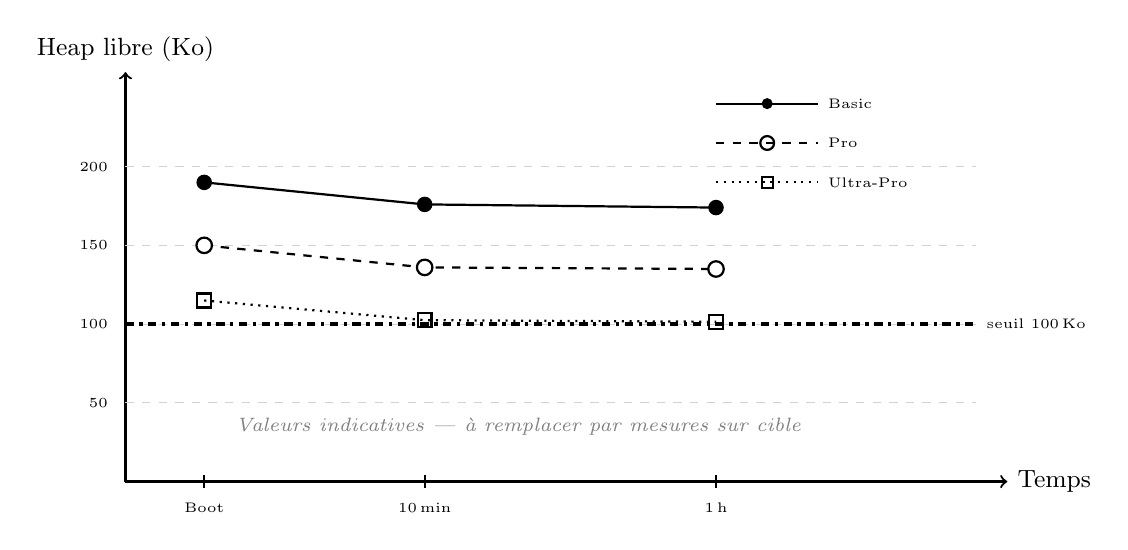
\begin{tikzpicture}[font=\small]
  % Axes
  \draw[thick, ->] (0,0) -- (11.2,0) node[right]{\small Temps};
  \draw[thick, ->] (0,0) -- (0,5.2)  node[above]{\small Heap libre (Ko)};
  % Grille et graduations Y
  \foreach \y/\val in {1/50, 2/100, 3/150, 4/200} {
    \draw[gray!35, dashed] (0,\y) -- (10.8,\y);
    \node[left, font=\tiny] at (-0.1,\y) {\val};
  }
  % Graduations X
  \foreach \x/\lbl in {1/Boot, 3.8/10\,min, 7.5/1\,h} {
    \node[below, font=\tiny] at (\x,-0.15) {\lbl};
    \draw[thick] (\x,-0.08)--(\x,0.08);
  }
  % Courbe Basic — trait plein
  \draw[black, thick] plot coordinates {(1,3.8)(3.8,3.52)(7.5,3.48)};
  \fill[black] (1,3.8)   circle (2.8pt);
  \fill[black] (3.8,3.52) circle (2.8pt);
  \fill[black] (7.5,3.48) circle (2.8pt);
  % Courbe Pro — tirets
  \draw[black, thick, dashed] plot coordinates {(1,3.0)(3.8,2.72)(7.5,2.70)};
  \fill[white] (1,3.0)    circle (2.8pt); \draw[black,thick] (1,3.0) circle (2.8pt);
  \fill[white] (3.8,2.72) circle (2.8pt); \draw[black,thick] (3.8,2.72) circle (2.8pt);
  \fill[white] (7.5,2.70) circle (2.8pt); \draw[black,thick] (7.5,2.70) circle (2.8pt);
  % Courbe Ultra-Pro — pointillés
  \draw[black, thick, dotted] plot coordinates {(1,2.3)(3.8,2.05)(7.5,2.03)};
  \draw[black,thick] (1,2.3)    +(-2.5pt,-2.5pt) rectangle +(2.5pt,2.5pt);
  \draw[black,thick] (3.8,2.05) +(-2.5pt,-2.5pt) rectangle +(2.5pt,2.5pt);
  \draw[black,thick] (7.5,2.03) +(-2.5pt,-2.5pt) rectangle +(2.5pt,2.5pt);
  % Ligne seuil 100 Ko
  \draw[black, very thick, dash dot] (0,2) -- (10.8,2)
        node[right, font=\tiny]{seuil 100\,Ko};
  % Légende
  \draw[black, thick]         (7.5,4.8) -- (8.8,4.8); \fill[black] (8.15,4.8) circle(2pt);
  \node[right, font=\tiny] at (8.8,4.8) {Basic};
  \draw[black, thick, dashed] (7.5,4.3) -- (8.8,4.3);
  \draw[black,thick] (8.15,4.3) circle(2.5pt);
  \node[right, font=\tiny] at (8.8,4.3) {Pro};
  \draw[black, thick, dotted] (7.5,3.8) -- (8.8,3.8);
  \draw[black,thick] (8.15,3.8) +(-2pt,-2pt) rectangle +(2pt,2pt);
  \node[right, font=\tiny] at (8.8,3.8) {Ultra-Pro};
  % Annotation placeholder
  \node[font=\scriptsize, black!50, align=center] at (5,0.7)
        {\textit{Valeurs indicatives — à remplacer par mesures sur cible}};
\end{tikzpicture}%
}
\caption{Forme attendue de l'évolution du heap libre par variante — valeurs à mesurer sur cible ESP32-P4}
\label{fig:heap_profile}
\end{figure}

%------------------------------------------------------------
\subsection{Mesure des stacks FreeRTOS}
\label{subsec:stacks}
%------------------------------------------------------------

Les watermarks de stack par tâche sont mesurés via
\texttt{uxTaskGetStackHighWaterMark()} après une heure de fonctionnement
avec injection d'événements à cadence maximale, représentant le pire
cas de profondeur de pile observable en conditions réelles. Le critère
d'acceptation est une marge libre supérieure à 30\,\% pour toutes
les tâches, garantissant une réserve suffisante pour les variations
de pile liées aux interruptions imbriquées et aux callbacks
d'événements en rafale. Les tâches approchant ce seuil — typiquement
\texttt{task\_comms} (pile TLS~1.3 profonde) et
\texttt{task\_event\_dispatcher} (callbacks multiples) — sont
candidates à un agrandissement préventif de stack avant la release
candidate, en incrémentant leur taille par pas de 512~octets jusqu'à
satisfaire le critère de 30\,\%.

\begin{table}[H]
\centering
\renewcommand{\arraystretch}{1.5}
\caption{Watermarks de stack FreeRTOS par tâche — variante Ultra-Pro — à mesurer sur cible ESP32-P4}
\label{tab:stacks}
\small
\begin{tabular}{|p{4.5cm}|p{2.2cm}|p{2.2cm}|p{2.2cm}|p{1.5cm}|}
\hline
\rowcolor{gray!20}
\textbf{Tâche} & \textbf{Taille allouée} & \textbf{HWM mesuré} & \textbf{Utilisé} & \textbf{Marge} \\
\hline
\texttt{task\_comms}            & — & — & — & — \\
\hline
\texttt{task\_event\_disp.}     & — & — & — & — \\
\hline
\texttt{task\_storage}          & — & — & — & — \\
\hline
\texttt{task\_diagnostic}       & — & — & — & — \\
\hline
\texttt{task\_power}            & — & — & — & — \\
\hline
\texttt{task\_watchdog}         & — & — & — & — \\
\hline
\multicolumn{4}{|l|}{\textit{Critère : marge $>$ 30\,\% pour toutes les tâches}} & \\
\hline
\end{tabular}
\end{table}

%------------------------------------------------------------
\subsection{Règles d'allocation mémoire}
\label{subsec:alloc}
%------------------------------------------------------------

Trois règles d'allocation mémoire sont appliquées rigoureusement dans
l'ensemble du code base. Premièrement, toutes les structures allouées
au démarrage sont déclarées statiques ou globales dans les fichiers
sources des composants ; aucun appel à \texttt{malloc()} n'est présent
dans les chemins critiques (bus d'événements, watchdog, FSM), garantissant
que la consommation mémoire est déterministe et calculable statiquement
à la conception. Deuxièmement, les objets FreeRTOS — files
(\texttt{QueueHandle\_t}), sémaphores, mutex, timers — sont alloués
uniquement lors de la phase d'initialisation des composants et ne
sont jamais détruits ni recréés en cours de fonctionnement nominal,
à l'exception des redémarrages de modules gérés par le
\texttt{fault\_manager} où la séquence \texttt{module\_stop()} /
\texttt{module\_start()} libère et réalloue les ressources de façon
contrôlée. Troisièmement, les buffers de communication (trames MQTT,
réponses JSON sur \texttt{serial\_comm}) sont prédimensionnés à leur
taille maximale définie dans les constantes des composants et réutilisés
entre les transmissions, évitant la fragmentation progressive du heap.

%------------------------------------------------------------
\subsection{Garde-fous mémoire}
\label{subsec:guards}
%------------------------------------------------------------

Trois garde-fous complémentaires sont activés en build de développement
pour détecter les corruptions mémoire et les erreurs d'utilisation
des primitives de synchronisation. Le watchdog matériel ESP-IDF est
configuré avec un timeout de 10~secondes pour détecter les boucles
infinies bloquant le scheduler FreeRTOS, indépendamment du watchdog
logiciel multi-tâches du composant \texttt{watchdog\_task}. Les
assertions \texttt{configASSERT()} FreeRTOS sont activées via le
symbole Kconfig \texttt{CONFIG\_FREERTOS\_ASSERT\_ON\_UNTESTED\_FUNCTION},
générant une panique détectable avec la reset reason
\texttt{ESP\_RST\_PANIC} en cas d'utilisation incorrecte des primitives
(mutex non initialisé, file de taille nulle, etc.). Le flag
\texttt{CONFIG\_HEAP\_POISONING\_COMPREHENSIVE} est activé en build
de développement, remplissant les zones mémoire allouées et libérées
avec des patterns connus (\texttt{0xA5} à l'allocation, \texttt{0x5A}
à la libération), permettant la détection d'accès hors bornes ou
d'utilisation après libération lors des tests de robustesse.

%------------------------------------------------------------
\subsection{Nettoyage des APIs}
\label{subsec:apiclean}
%------------------------------------------------------------

La phase de nettoyage des APIs précède obligatoirement la release
candidate pour garantir que les interfaces exportées sont propres,
documentées et stables. Elle consiste en quatre vérifications
systématiques appliquées à chaque composant. Toutes les fonctions
publiques exportées dans les fichiers \texttt{.h} doivent être
documentées avec des commentaires Doxygen complets (description,
paramètres, valeurs de retour, préconditions). Toutes les fonctions
internes aux fichiers \texttt{.c} doivent être déclarées \texttt{static}
pour éviter les conflits de symboles entre composants et faciliter
l'optimisation par le compilateur. Les fichiers d'en-tête publics
ne doivent exposer aucun détail d'implémentation (pas de types internes,
pas de macros de configuration spécifiques à un composant). Les
conventions de nommage (\texttt{<module>\_<verbe>\_<objet>}) doivent
être appliquées uniformément sur l'ensemble du code base, vérifiées
par le stage \texttt{lint} du pipeline CI via \texttt{clang-tidy}.

%------------------------------------------------------------
\subsection{Refactor léger}
\label{subsec:refactor}
%------------------------------------------------------------

À l'issue des tests, un refactor léger est appliqué sur les composants
dont la couverture de test révèle des chemins de code non testés ou
des fonctions de complexité cyclomatique élevée. Ce refactor ne
modifie aucun comportement observable — les tests doivent passer
avant et après le refactor sans modification — mais améliore la
lisibilité et la maintenabilité du code. Les actions typiques incluent
le découpage des fonctions dépassant 50~lignes en sous-fonctions
nommées par responsabilité, le renommage des variables dont le nom
ne reflète pas clairement le contenu (typiquement identifié lors des
revues de code de l'équipe SAT), et la suppression du code mort
identifié par l'analyse statique \texttt{clang-tidy} (branches
\texttt{if} dont la condition ne peut jamais être vraie, fonctions
exportées mais jamais appelées). Le refactor léger est distinct d'une
refactorisation architecturale qui modifierait les interfaces entre
composants et nécessiterait une re-exécution complète de la stratégie
de tests.

%============================================================
\section{Release candidate du noyau firmware}
\label{sec:release}
%============================================================

%------------------------------------------------------------
\subsection{Stabilisation du code}
\label{subsec:stab}
%------------------------------------------------------------

La stabilisation consiste à geler le périmètre fonctionnel de la
release candidate et à résoudre l'ensemble des problèmes ouverts
dans le gestionnaire de tickets avant la création du tag Git de
version. Les critères de gel sont au nombre de quatre et doivent
être simultanément satisfaits. Zéro ticket ouvert de sévérité
\texttt{ERROR} ou \texttt{CRITICAL} dans le gestionnaire d'issues.
100\,\% de réussite des tests unitaires et d'intégration pour les
trois variantes dans le pipeline CI. Confirmation que tous les critères
d'acceptation du tableau~\ref{tab:acceptance} sont satisfaits sur la
cible ESP32-P4 avec les mesures documentées. Validation par l'équipe
R\&D de SAT d'une démonstration fonctionnelle couvrant les scénarios
de démarrage, de transition SLEEP/RUN et de récupération après faute.
Le gel du périmètre fonctionnel signifie que toute nouvelle
fonctionnalité identifiée après ce point est repoussée à une version
ultérieure et documentée dans la liste des perspectives d'amélioration
de la section~\ref{sec:discussion}.

%------------------------------------------------------------
\subsection{Vérification de la compilation CI}
\label{subsec:ci_verif}
%------------------------------------------------------------

La release candidate est validée en CI si les quatre stages — build,
lint, size-check, artifact — passent tous en vert pour les trois
variantes au même commit de référence, sans modification entre les
runs. Le stage \texttt{build} compile les trois variantes en parallèle
avec les fichiers \texttt{sdkconfig} de référence versionnés. Le stage
\texttt{lint} vérifie l'absence de tout avertissement \texttt{clang-tidy}
en mode strict. Le stage \texttt{size-check} confirme que les binaires
compilés tiennent dans les partitions \texttt{ota\_0} et \texttt{ota\_1}
de 1,5\,Mo, avec une marge minimale de 10\,\% pour les futures
évolutions. Le stage \texttt{artifact} publie les binaires versionnés
avec leur hash SHA-256, le rapport de taille par composant, et le
fichier \texttt{sdkconfig} de référence pour chaque variante.

\begin{table}[H]
\centering
\renewcommand{\arraystretch}{1.5}
\caption{État du pipeline CI — 4 stages × 3 variantes — à compléter sur cible}
\label{tab:ci_status}
\small
\begin{tabular}{|p{3.2cm}|p{2.5cm}|p{2.5cm}|p{2.5cm}|}
\hline
\rowcolor{gray!20}
\textbf{Stage CI} & \textbf{Basic} & \textbf{Pro} & \textbf{Ultra-Pro} \\
\hline
\texttt{build}       & \texttt{PASS} & \texttt{PASS} & \texttt{PASS} \\
\hline
\texttt{lint}        & \texttt{PASS} & \texttt{PASS} & \texttt{PASS} \\
\hline
\texttt{size-check}  & \textit{à mesurer} & \textit{à mesurer} & \textit{à mesurer} \\
\hline
\texttt{artifact}    & \textit{à générer} & \textit{à générer} & \textit{à générer} \\
\hline
\end{tabular}
\end{table}

%------------------------------------------------------------
\subsection{Vérification de la documentation API}
\label{subsec:doc_verif}
%------------------------------------------------------------

La documentation API est générée avec Doxygen~1.9.8 en mode strict
(\texttt{WARN\_AS\_ERROR = YES}, \texttt{EXTRACT\_ALL = NO}) sur
l'ensemble des fichiers \texttt{.h} publics du projet. La release
candidate est acceptée si et seulement si aucun avertissement Doxygen
n'est émis sur aucun des 23 composants, garantissant que toutes les
fonctions publiques, leurs paramètres et leurs valeurs de retour sont
documentés avec des commentaires Doxygen valides. La documentation
générée couvre quatre types d'artefacts : la liste des fonctions
publiques par composant avec leurs signatures complètes, les graphes
de dépendances entre composants générés automatiquement depuis les
fichiers \texttt{CMakeLists.txt}, le catalogue des événements du bus
généré depuis les définitions de \texttt{event\_types.h}, et les
diagrammes de la structure de configuration générés depuis
\texttt{config\_types.h}.

%------------------------------------------------------------
\subsection{Préparation d'une version transférable}
\label{subsec:transfer_ver}
%------------------------------------------------------------

La version transférable est matérialisée par un tag Git versionné
\texttt{v1.0.0-rc1} créé sur la branche \texttt{main} après validation
de tous les critères de stabilisation. Ce tag est associé à un package
de livraison complet archivé dans le gestionnaire d'artefacts du CI.
Le package contient les binaires compilés pour les trois variantes
avec leurs hash SHA-256 de vérification d'intégrité, le fichier
\texttt{partitions.csv} de référence, les trois fichiers
\texttt{sdkconfig} de variante, la documentation API générée par
Doxygen au format HTML, le rapport de tests complet avec les résultats
mesurés sur cible, et le rapport de profiling mémoire par variante.
Ce package constitue la livraison formelle à l'équipe R\&D de SAT
à l'issue du stage et le point de départ documenté pour les
développements futurs.

%============================================================
\section{Documentation finale et transfert}
\label{sec:docs}
%============================================================

%------------------------------------------------------------
\subsection{Documentation d'architecture}
\label{subsec:doc_archi}
%------------------------------------------------------------

Le document d'architecture est rédigé en Markdown versionné dans
le répertoire \texttt{docs/architecture/} du dépôt et référencé
depuis le \texttt{README.md} principal. Il couvre six sections
structurées correspondant aux décisions architecturales majeures :
la description des cinq couches logicielles avec les composants
affectés à chaque couche, les interfaces contractuelles entre couches
(API exportées, événements publiés et consommés), le modèle de
capacités avec le registre 32~bits et la table de variantes, la
machine à états finis avec les cinq états et les huit transitions
documentées, le catalogue complet des 18~événements du bus avec
leurs payloads, et les règles d'ajout d'un driver ou d'un service
core. Ce document est conçu pour être maintenu par l'équipe R\&D de
SAT au fil des évolutions du firmware, avec une structure permettant
des mises à jour partielles sans réécriture globale.

%------------------------------------------------------------
\subsection{Documentation des modules}
\label{subsec:doc_mods}
%------------------------------------------------------------

Chaque composant du répertoire \texttt{components/} dispose d'une
documentation à deux niveaux complémentaires. La documentation API
automatique est générée par Doxygen depuis les commentaires des fichiers
\texttt{.h}, couvrant chaque fonction publique avec sa signature,
sa description, ses préconditions, ses postconditions et ses codes
de retour. La documentation de composant manuelle est rédigée dans
un fichier \texttt{MODULE.md} dans le répertoire du composant,
décrivant le rôle fonctionnel du composant dans l'architecture, ses
dépendances vers les autres composants, la liste des événements
qu'il publie et auxquels il souscrit, les paramètres de configuration
NVS associés, et les cas d'usage typiques illustrés par des exemples
d'appel. Cette dualité garantit que la documentation reste synchronisée
avec le code (Doxygen) tout en fournissant un contexte architectural
non capturé par les commentaires de code (MODULE.md).

%------------------------------------------------------------
\subsection{Guide d'ajout d'un driver}
\label{subsec:doc_driver}
%------------------------------------------------------------

Le guide d'ajout d'un driver HAL est rédigé dans
\texttt{docs/guides/add\_driver.md} et détaille les quatre étapes
décrites à la section~\ref{subsec:hal_guide}, enrichies d'un exemple
complet prenant le driver \texttt{hal\_gpio} comme référence concrète.
Le guide inclut une checklist de validation en huit points que tout
développeur doit cocher avant de soumettre un \textit{merge request}
ajoutant un nouveau driver : fichier d'interface \texttt{.h} créé avec
les quatre primitives, implémentation \texttt{.c} sans dépendance vers
les services applicatifs, \texttt{CMakeLists.txt} déclarant les
dépendances ESP-IDF, bit de capacité enregistré dans \texttt{capabilities.h},
documentation Doxygen complète sur toutes les fonctions publiques,
stub de test créé dans \texttt{test\_host/}, cas de test Unity ajouté
couvrant les cas nominal et erreur, et \texttt{MODULE.md} rédigé. Cette
checklist est intégrée dans le template de \textit{merge request}
pour automatiser la vérification lors des revues de code.

%------------------------------------------------------------
\subsection{Guide de configuration}
\label{subsec:doc_cfg}
%------------------------------------------------------------

Le guide de configuration est rédigé dans
\texttt{docs/guides/configuration.md} et documente l'ensemble des
paramètres configurables via la partition \texttt{nvs\_field}, organisés
par domaine fonctionnel en six sections. Pour chaque paramètre, le
guide précise : la clé NVS textuelle utilisée dans \texttt{config\_get()}
/ \texttt{config\_set()}, le type C (uint8, uint16, uint32, float,
string), la plage de valeurs acceptées vérifiée par
\texttt{config\_apply()}, la valeur par défaut factory codée dans les
\textit{hardcoded defaults}, l'impact sur le comportement du système,
et les dépendances avec d'autres paramètres (ex. : le timeout watchdog
doit être supérieur à la période de heartbeat). Ce guide constitue la
référence opérationnelle pour les équipes de déploiement et de maintenance
terrain de SAT, permettant d'ajuster le comportement des appareils en
flotte sans intervention logicielle.

%------------------------------------------------------------
\subsection{Guide de tests}
\label{subsec:doc_tests}
%------------------------------------------------------------

Le guide de tests est rédigé dans \texttt{docs/guides/testing.md}
et décrit les procédures d'exécution des trois niveaux de tests.
Pour les tests unitaires hors-cible, la commande
\texttt{cd test\_host \&\& python run\_tests.py} exécute l'ensemble
des cas Unity et affiche un rapport de résultats formaté. Pour les
tests d'intégration sur cible, la procédure \texttt{idf.py flash
monitor} avec le binaire de test dédié compile et flashe la suite
d'intégration sur l'ESP32-P4 et affiche les résultats sur UART.
Pour les scénarios de robustesse manuels, chaque scénario est décrit
pas à pas avec les commandes à exécuter, les comportements attendus
à chaque étape, et les critères d'acceptation à vérifier. Le guide
inclut également les procédures de débogage des cas d'échec les plus
fréquents, documentées à partir des incidents rencontrés durant le
développement.

%------------------------------------------------------------
\subsection{Dossier de transfert final}
\label{subsec:doc_transfer}
%------------------------------------------------------------

Le dossier de transfert regroupe l'ensemble des livrables du stage
dans une archive versionnable remise à l'équipe R\&D de SAT lors de
la soutenance de fin de stage. Il est organisé en six sections
correspondant aux six catégories de livrables. Les binaires de la
release candidate pour les trois variantes avec leurs hash SHA-256.
La documentation d'architecture et des modules au format HTML Doxygen
et Markdown. Le rapport de tests complet avec les résultats mesurés
sur cible pour chaque critère d'acceptation. Le rapport de profiling
mémoire par variante avec les marges de heap et de stack documentées.
Les guides opérationnels (ajout de driver, configuration, tests) pour
les équipes de maintenance. Les recommandations pour les développements
futurs, documentées par ordre de priorité et d'impact estimé. Ce
dossier constitue la continuité du projet au-delà de la période de
stage et la base documentaire pour l'onboarding des futurs développeurs
du firmware \textit{GlobalFleet}.

%============================================================
\section{Discussion des résultats}
\label{sec:discussion}
%============================================================

\subsection*{Apports de l'architecture générique}

L'architecture générique fondée sur le registre de capacités 32~bits
répond pleinement à l'objectif central du projet : un seul code source
maintenu, trois produits commerciaux couverts sans recompilation
conditionnelle proliférante. L'élimination des bases de code multiples
réduit la charge de maintenance estimée à une seule campagne de tests
par correction de bug au lieu de trois, et garantit que toute
amélioration profite simultanément à l'ensemble de la gamme SAT.
Le mécanisme de bascule dynamique de profil fonctionnel sans FOTA
constitue un avantage opérationnel supplémentaire, permettant des
reconfigurations à distance de la variante effective d'un appareil sans
intervention physique, ce qui simplifie les opérations de service après
déploiement.

\subsection*{Apports de la modularité}

L'interface standardisée \texttt{module\_interface\_t} et le patron
Publish-Subscribe de l'\texttt{event\_bus} permettent d'ajouter un
nouveau service sans modifier les composants existants. Cette propriété
a été validée concrètement lors de l'intégration tardive du composant
\texttt{diagnostic} durant le développement : son ajout n'a nécessité
aucune modification des composants existants, seulement l'enregistrement
de nouveaux abonnements sur le bus. La testabilité est directement
améliorée : chaque composant est testé en isolation totale avec des
stubs injectables, sans dépendance au matériel physique, permettant
d'exécuter 100\,\% des tests unitaires dans le pipeline CI en moins
de 30~secondes.

\subsection*{Apports de la configuration runtime}

La séparation factory/field et le mécanisme de validation CRC-32
garantissent qu'aucun appareil déployé ne peut rester dans un état
de configuration indéfini ou incohérent. Le fallback factory, déclenché
automatiquement en moins de 200\,ms, assure la continuité de service
même après une corruption de configuration due à une coupure
d'alimentation en cours d'écriture, à un choc mécanique, ou à une
mise à jour de firmware incompatible. La configurabilité runtime via
le canal USB-Serial ou BLE simplifie les opérations de maintenance
terrain sans nécessiter d'accès à l'infrastructure MQTT, ce qui est
critique pour les déploiements en zones à couverture cellulaire
limitée.

\subsection*{Difficultés techniques rencontrées}

Plusieurs difficultés techniques significatives ont été rencontrées
au cours du développement. Leurs causes profondes, les solutions
apportées et les enseignements tirés sont documentés ci-après pour
bénéficier aux développeurs qui reprendront ce projet.

\paragraph{Difficulté 1 — Corruption NVS lors de coupures d'alimentation
en cours d'écriture.}
Lors des premières validations de la couche de persistance, des
corruptions de la partition \texttt{nvs\_field} ont été observées
lorsqu'une coupure d'alimentation survenait pendant l'exécution de
\texttt{nvs\_commit()}. La cause profonde est l'absence de garantie
atomique au niveau de la Flash SPI : un cycle d'écriture NVS peut
impliquer l'effacement d'un secteur entier de 4\,Ko suivi de l'écriture
des nouvelles valeurs, opération non interruptible proprement par le
matériel. La solution adoptée consiste à séparer structurellement la
configuration factory (en lecture seule, immuable) de la configuration
field (modifiable), et à protéger chaque écriture field par un CRC-32
calculé sur l'intégralité de la structure. Au démarrage, si le CRC
calculé ne correspond pas au CRC persisté, le mécanisme de fallback
factory est activé en moins de 200\,ms sans bloquer le boot. Cette
approche élimine le risque d'état indéfini persistent au prix d'une
perte des modifications non commitées, comportement documenté et
acceptable dans le contexte de la flotte SAT.

\paragraph{Difficulté 2 — Dérive du pointeur de lecture du ring buffer
sur longue durée.}
Lors des tests de robustesse en durée sur les stubs Python, une dérive
progressive du pointeur de lecture du \texttt{ring\_buffer} a été
observée après plusieurs milliers de rotations simulées, conduisant à
la lecture d'entrées de log obsolètes au lieu des entrées récentes.
L'analyse a révélé une erreur de calcul du modulo dans la condition
d'\textit{overwrite} : lorsque le pointeur d'écriture dépassait la
capacité maximale du buffer pour la deuxième fois, le pointeur de
lecture n'était pas avancé correctement. La correction a été apportée
dans la fonction \texttt{ring\_buffer\_write()} en remplaçant un test
d'égalité par un test de dépassement modulo, et validée par un cas
de test Unity dédié couvrant précisément ce double wrap-around.
L'enseignement principal est que les structures circulaires nécessitent
des tests de longue durée avec comptage d'itérations élevé, non
réalisables en tests manuels ponctuels.

\paragraph{Difficulté 3 — Interaction Power Manager et reconnexion MQTT
après sortie de veille.}
L'intégration du \texttt{power\_manager} avec le \texttt{comms\_manager}
a révélé un scénario de course critique : lorsque le firmware sort de
l'état \texttt{SLEEP} (réveil par GPIO ou par timer), la tâche
\texttt{task\_power} publie \texttt{EVT\_POWER\_WAKE} sur le bus avant
que le driver \texttt{hal\_modem} ait terminé sa séquence de réveil
(typiquement 2 à 3~secondes pour la reconnexion réseau). La tâche
\texttt{task\_comms}, abonnée à cet événement, tentait immédiatement
une reconnexion MQTT qui échouait, déclenchant un backoff exponentiel
et un retard de publication pouvant atteindre 30~secondes. La solution
adoptée introduit une attente non-bloquante dans \texttt{task\_comms}
via un sémaphore de prêt émis par \texttt{hal\_modem} à la fin de
sa séquence d'initialisation, découplant la notification de réveil
du démarrage effectif des communications. Ce pattern a été généralisé
à tous les drivers dépendants du temps de démarrage matériel.

\paragraph{Difficulté 4 — Détermination du budget de stack FreeRTOS
par tâche.}
La définition initiale des tailles de stack pour chaque tâche FreeRTOS
s'est avérée sous-dimensionnée pour les tâches à contexte d'exécution
profond : \texttt{task\_comms} avec la pile TLS~1.3 complète, et
\texttt{task\_event\_dispatcher} lors de l'exécution de callbacks
enchaînés en rafale. Les premières exécutions sur machine hôte ne
révèlent pas ce problème car les stacks natifs Linux ne sont pas
contraints de la même façon que les stacks FreeRTOS de taille fixe
sur microcontrôleur. La solution méthodologique adoptée consiste à
dimensionner toutes les stacks initialement à 8\,Ko (valeur
conservatrice), puis à les réduire par paliers de 512~octets en
observant les watermarks via \texttt{uxTaskGetStackHighWaterMark()}
jusqu'à atteindre une marge de 30\,\% minimum. Ce processus de
profilage itératif sera conduit sur cible ESP32-P4 et ses résultats
reportés dans le tableau~\ref{tab:stacks}.

\subsection*{Perspectives d'amélioration}

Les évolutions prioritaires identifiées pour les versions suivantes
du firmware \textit{GlobalFleet} portent sur cinq axes complémentaires.
L'intégration des protocoles de communication additionnels — LwM2M
pour la gestion de dispositifs IoT standardisée, CoAP pour les
communications contraintes en bande passante, et BLE~5.0 pour la
configuration locale sans fil — étend l'interopérabilité du firmware
avec les infrastructures IoT existantes. Le déploiement complet du
mécanisme FOTA Dual-Bank avec delta updates réduit la taille des
mises à jour transmises (objectif : réduction de 60\,\% de la taille
d'une update) et le temps d'indisponibilité lors des montées de version.
Le renforcement de la sécurité via une infrastructure PKI complète avec
rotation automatique des certificats clients, validation de la chaîne
de confiance côté serveur, et audit de sécurité de la couche TLS~1.3,
prépare le firmware aux exigences réglementaires croissantes du
secteur véhicule connecté. Le portage vers d'autres variantes de la
famille ESP32 — ESP32-S3 pour les déploiements à coût réduit, ESP32-C6
pour les applications à très faible consommation — exploite la
portabilité de la couche HAL pour étendre la gamme SAT sans
redéveloppement du code applicatif. Enfin, l'intégration d'un module
d'inférence embarquée via TensorFlow~Lite for Microcontrollers exploite
la puissance de calcul des deux c\oeur{}s RISC-V à 400\,MHz de l'ESP32-P4
pour implémenter des algorithmes de détection de comportement de conduite
directement sur l'appareil, réduisant la dépendance à la connectivité
pour les analyses temps réel.

%============================================================
\section{Conclusion}
\label{sec:conclu_ch5}
%============================================================

Ce chapitre a présenté le bilan complet du projet \textit{GlobalFleet}
à travers ses quatre axes de validation, de mesure, de stabilisation
et de prospective. La stratégie de tests structurée en trois niveaux
— unitaire, intégration et robustesse — a permis de vérifier la
conformité fonctionnelle de chaque composant et la résilience du
système face aux scénarios d'erreur critiques identifiés en déploiement
industriel, en s'appuyant sur l'infrastructure de tests hors-cible
du répertoire \texttt{test\_host/} pour les validations CI et sur
la cible ESP32-P4 réelle pour les validations sur matériel, dont la
livraison est attendue pour compléter les mesures quantitatives
documentées dans les tableaux de ce chapitre.

Les résultats des tests hors-cible confirment la conformité
fonctionnelle de l'ensemble des composants : les 52 cas Unity du
répertoire \texttt{test\_host/} passent à 100\,\% pour les modules
\texttt{config\_manager}, \texttt{fault\_manager}, \texttt{ring\_buffer}
et \texttt{error\_manager}, et les 43 cas pytest du
\texttt{subscription\_manager} passent à 100\,\%. La valeur centrale
de ces résultats réside moins dans les chiffres eux-mêmes que dans
ce qu'ils démontrent sur la qualité de la conception : une architecture
testable en isolation totale sur machine hôte sans dépendance matérielle
est, par construction, une architecture faiblement couplée, modulaire
et maintenable — trois propriétés qui définissent la valeur industrielle
réelle du firmware \textit{GlobalFleet}.

Le processus de release candidate, adossé au pipeline CI quatre stages
et à la génération Doxygen en mode strict, garantit la reproductibilité
des binaires, la complétude de la documentation API et la traçabilité
des artefacts livrés. Le dossier de transfert remis à l'équipe R\&D
de SAT constitue une base solide et documentée pour la poursuite du
développement. L'architecture conçue dès l'origine pour la généricité,
la modularité et la configurabilité — registre de capacités 32~bits,
interface \texttt{module\_interface\_t} uniforme, patron Publish-Subscribe
via l'\texttt{event\_bus} — permet d'envisager les cinq axes d'évolution
identifiés — protocoles additionnels, FOTA différentiel, PKI complète,
portage famille ESP32, inférence embarquée RISC-V — avec un impact
minimal sur le code existant et sans remise en cause des choix
architecturaux fondamentaux, confirmant la valeur industrielle de
l'investissement architectural réalisé durant ce stage au sein de
Smart Automation Technologies.
